
%! program = pdflatex

\documentclass[12pt]{article}
\usepackage{amsmath}
\usepackage{natbib}
\usepackage{graphicx}
\usepackage{amssymb}
\usepackage{epstopdf}
\usepackage{float} % to keep the figures in place
\usepackage{placeins}

\usepackage{caption}
\usepackage{subcaption}
\usepackage{color}
%\usepackage{undertilde}
\usepackage{enumitem}
\newcommand{\cred}{ \color{red}}
\newcommand{\cgreen}{\color{green}}
\newcommand{\cblue}{\color{blue}}
\newcommand{\cmag}{\color{magenta}}
\newcommand{\bn}{\begin{enumerate}}
\newcommand{\en}{\end{enumerate}}
\newcommand{\bi}{\begin{itemize}}
\newcommand{\ei}{\end{itemize}}
\newcommand{\be}{\begin{eqnarray}}
\newcommand{\ee}{\end{eqnarray}}
\newcommand{\by}{\begin{eqnarray*}}
\newcommand{\ey}{\end{eqnarray*}}
\renewcommand{\labelenumi}{(\alph{enumi}) }
%
\usepackage[margin=2.2cm, includehead]{geometry}% see geometry.pdf on how to lay out the page. There's lots.
\geometry{letterpaper} % or letter or a5paper or ... etc
% \geometry{landscape} % rotated page geometry
%\bibpunct{(}{)}{;}{a}{,}{,}
%\setlength{\textwidth}{16cm}
%\setlength{\textheight}{21cm}
\def\nonumber{\global\@eqnswfalse}
\newcounter{parnum}
\newcommand{\N}{%
  \noindent\refstepcounter{parnum}%
   \makebox[\parindent][l]{\textbf{[\arabic{parnum}]}}\quad  }
% Use a generous paragraph indent so numbers can be fit inside the
% indentation space.
\setlength{\parindent}{1.5em}

% See the ``Article customise'' template for come common customisations

\date{}
%\date{} % delete this line to display the current date

%%% BEGIN DOCUMENT
\begin{document}
\SweaveOpts{concordance=TRUE}
%\large
%\maketitle
\newtheorem{thm}{Theorem}[section]
\newtheorem{cor}[thm]{Corollary}
\newtheorem{lem}[thm]{Lemma}
\newtheorem{prop}[thm]{Proposition}
\newtheorem{defn}[thm]{Definition}
\newtheorem{exam}[thm]{Example}
\newtheorem{qstn}[thm]{Question}

%%%
\newpage
\begin{center}
{\bf Homework 2 - STAT 540}\\
Amal Agarwal
\end{center}
%==========================
\section*{Answer 1}
\begin{enumerate}[label=(\alph*)]
\item Psudocode:
\begin{itemize}
\item Let the unnormalized target kernel be $h(x)$. Evaluate the endpoints for the rectangle as $b=\sup_{x}(\sqrt{h(x)})$, $c=-\sup_{x}(x\sqrt{h(x)})$, and $d=\sup_{x}(x\sqrt{h(x)})$ using numerical maximization. 
\item Uniformly sample in 2 dimensions from the rectangle [$c\leq u\leq d] \times [0\leq v\leq b$].
\item For each sample pair (u,v), check the condition $0\leq v\leq h\left(\sqrt{\left(\dfrac{u}{v}\right)}\right)$ and keep only those pairs which satisfy the condition. Note that since the support is $(1,+\infty)$, we must have $u\geq v$.
\item Samples from the target density can be obtained by evaluating $\dfrac{u^{*}}{v^{*}}$ where $(u^{*},v^{*})$ are the accepted pairs from previous step.
\end{itemize}

\item R code for the algorithm is given in "aua257HW2.R" file.
\item Histogram of the samples along with true target kernel is given below:

\begin{knitrout}
\definecolor{shadecolor}{rgb}{0.969, 0.969, 0.969}\color{fgcolor}\begin{kframe}


{\ttfamily\noindent\itshape\color{messagecolor}{\#\# Loading required package: mvtnorm\\\#\# Loading required package: Matrix\\\#\# Loading required package: stats4\\\#\# Loading required package: gmm\\\#\# Loading required package: sandwich}}\end{kframe}
\end{knitrout}
\begin{figure}[H]
\begin{centering}
\begin{knitrout}
\definecolor{shadecolor}{rgb}{0.969, 0.969, 0.969}\color{fgcolor}\begin{kframe}


{\ttfamily\noindent\itshape\color{messagecolor}{\#\# stat\_bin: binwidth defaulted to range/30. Use 'binwidth = x' to adjust this.}}

{\ttfamily\noindent\color{warningcolor}{\#\# Warning: Removed 1 rows containing missing values (geom\_path).}}\end{kframe}
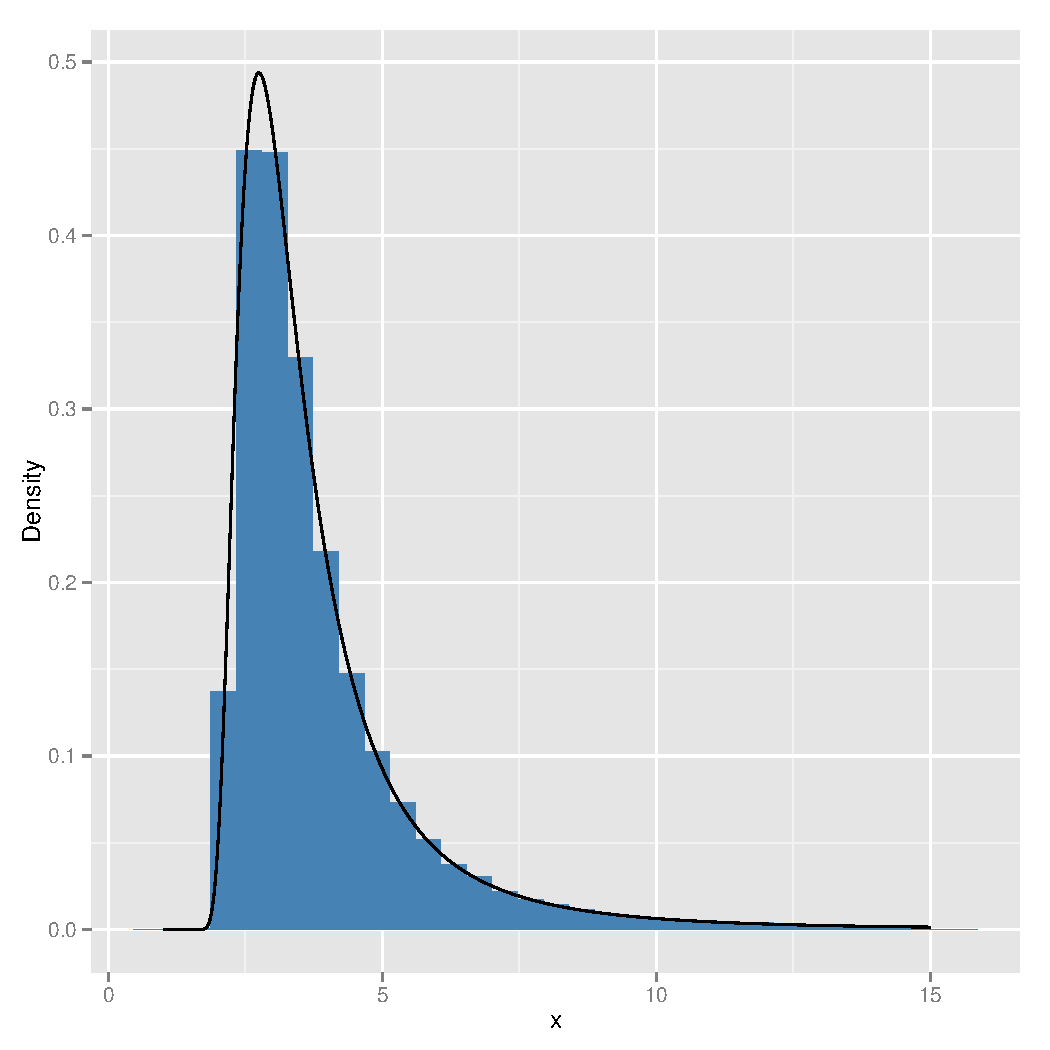
\includegraphics[width=\maxwidth]{figure/unnamed-chunk-2-1} 

\end{knitrout}
\caption{Plot of histogram of samples and comparing with true target kernel}
\end{centering}
\end{figure}
\clearpage
Plot of the ratio of uniforms of regions is given below:
\begin{figure}[H]
\begin{centering}
\begin{knitrout}
\definecolor{shadecolor}{rgb}{0.969, 0.969, 0.969}\color{fgcolor}
\includegraphics[width=\maxwidth]{figure/unnamed-chunk-3-1} 

\end{knitrout}
\caption{Plot of ratio of uniforms region}
\end{centering}
\end{figure}

\item The optimal sample size such that the Monte Carlo standard error is less than 5\% of the estimated expectation was found as \textbf{$248$}. This was obtained by running the ratio of uniforms function multiple items generating different sets of samples and calculating the optimal size in each case and taking the mean of the optimal sizes. 

The estimate of the expected value for $n=100,000$ was found as \textbf{3.98}.

Plot of the estimates of expected value with the sample size is given as:
\begin{figure}[H]
\begin{centering}
\begin{knitrout}
\definecolor{shadecolor}{rgb}{0.969, 0.969, 0.969}\color{fgcolor}
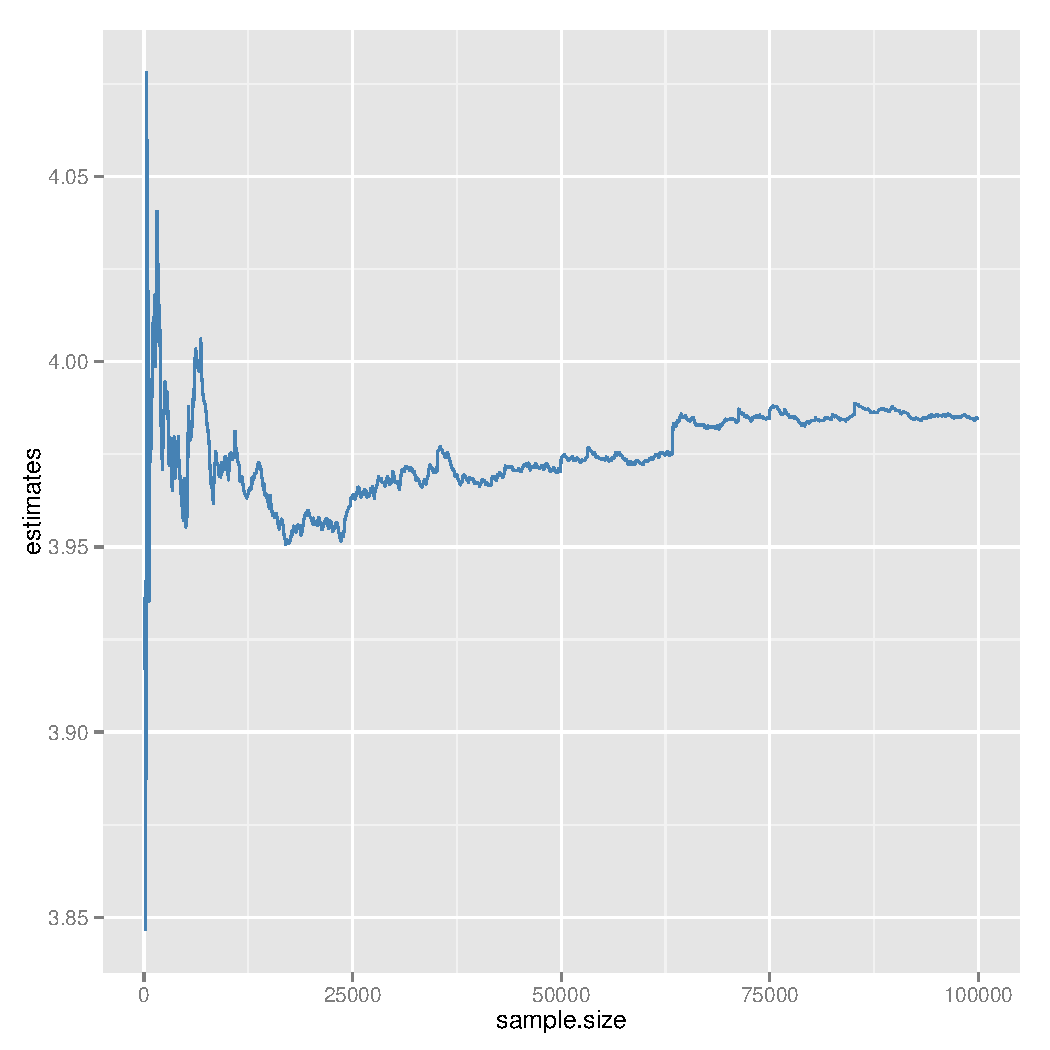
\includegraphics[width=\maxwidth]{figure/unnamed-chunk-4-1} 

\end{knitrout}
\caption{Plot of Monte Carlo estimates vs. sample size}
\end{centering}
\end{figure}
\clearpage
Plot of the Monte Carlo standard errors with the sample size is given as:
\begin{figure}[H]
\begin{centering}
\begin{knitrout}
\definecolor{shadecolor}{rgb}{0.969, 0.969, 0.969}\color{fgcolor}
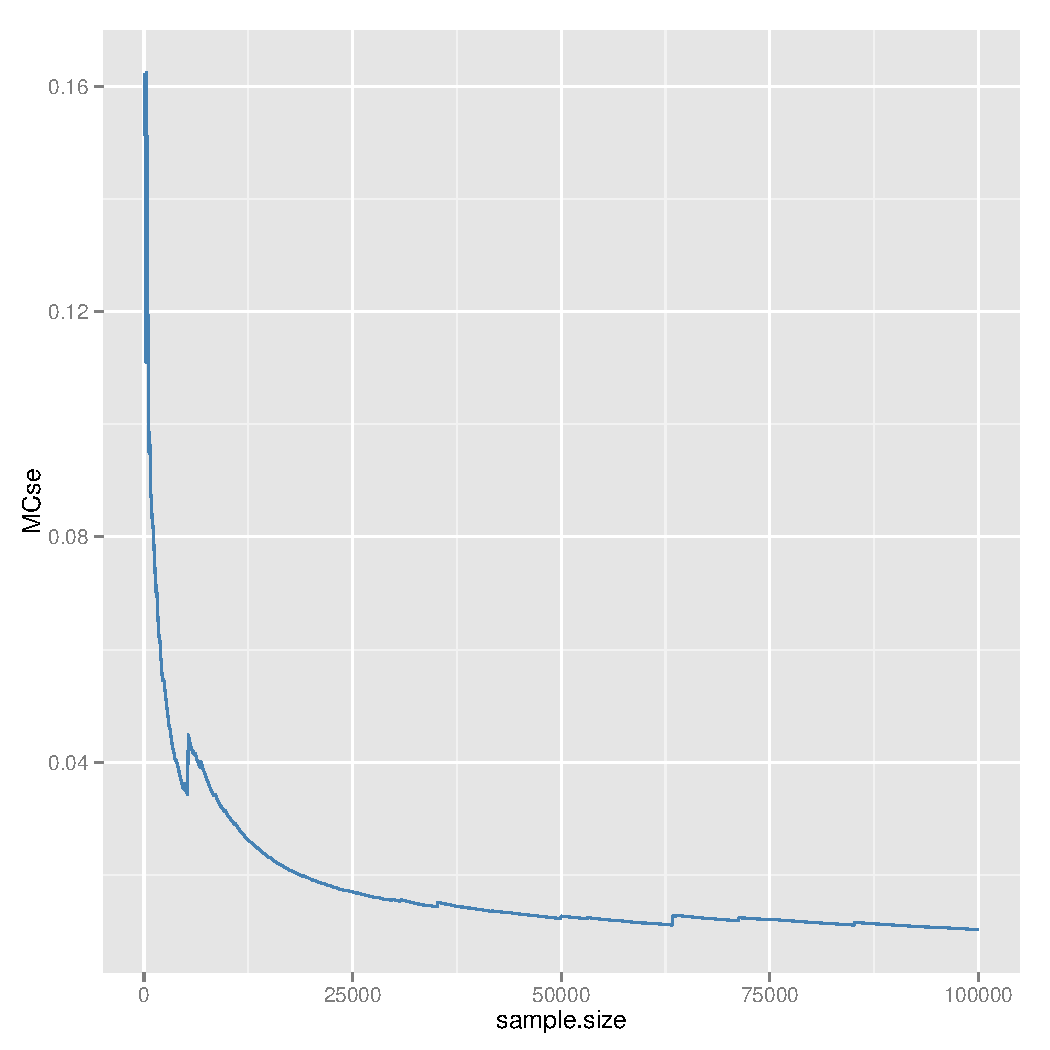
\includegraphics[width=\maxwidth]{figure/unnamed-chunk-5-1} 

\end{knitrout}
\caption{Plot of Monte Carlo standard errors vs. sample size}
\end{centering}
\end{figure}

\item The number of samples generated per second were found to be \textbf{\ensuremath{3.2884\times 10^{4}}}.

\end{enumerate}

%%%%%%%%%%%%%%%%%%%%%%%%%%%%%%%%%%%%%%%%%%%%%%%%%%%%%%%%%%%%%%%%%%%%%%%%%%%%%%%%%%%%%
\section*{Answer 2}
\begin{enumerate}[label=(\alph*)]
\item Refer to the file "aua257HW2.R" for R code. Pseudocode is given as follows:
\begin{itemize}
\item Start off with $x^{(0)}$ in the support $(1,+\infty)$ chosen suitably after a series of pilot runs. Choose the length of the Markov chain as $m$.
\item Run loop from $t=0:(m-1)$
\begin{itemize}
\item Generate a candidate $x^{*}$ from the propsal $q$ as truncated normal N($x^{(t)},\tau^2,1,+\infty$). For sampling $x^{*}$, inverse cdf transformation is being used as follows:
\begin{itemize}
\item Generate $u\sim Uniform(0,1)$.
\item To obtain $x^{*}$, do the inverse cdf transform on $u$ as $x_i^{*}=qnorm(u\times (pnorm(b_i)-pnorm(a_i)) +pnorm(a_i))$ where qnorm and pnorm are quantile and cdf functions for a normal distribution with parameters same as the mean and variance of $x^{*}$ defined above. 
\end{itemize}
\item Accept $x^{*}$ as next state $x^{(t+1)}$ with the following acceptance probability $\alpha$, else assign the current state as next state.
\[\alpha(x^{*},x^{(t)})=\text{min}\left(1,\dfrac{h(x^{*})q(x^{*},x^{t})}{h(x^{(t)})q(x^{t},x^{*})})\right)\]
where $h$ is the target kernel without the factor $(1/\sigma)$ in the target density.
\end{itemize}
\end{itemize}
































